\documentclass[12pt,letterpaper]{article}

\usepackage{caption} % for the figure captions
\usepackage[osf]{mathpazo} % a nicer font
% this is a package for the citation formats: found this formulation sorted natbib errors when changing packages
%from http://tex.stackexchange.com/questions/54480/package-natbib-error-bibliography-not-compatible-with-author-year-citations
\usepackage[square,sort,comma,numbers]{natbib} 
\usepackage{amsmath} % package for equations
\usepackage{url} % package for urls
\usepackage{hyperref} % for hyperlinks
\usepackage[a4paper, total={6in, 9in}]{geometry}
\hypersetup{
     colorlinks   = true,
     citecolor    = gray
}
\usepackage{graphicx} % for the figures
\usepackage{pdfpages}

\hypersetup{linkcolor=blue}

\pagenumbering{gobble}

\graphicspath{ }

\begin{document}

%title

{\Huge\textbf{\textit{Palaeospondylus}}\par}
\vspace{3mm}
{\large{Pay-lee-oh-spon-die-lus} \par} 
\vspace{5mm}
\textit{Palaeospondylus} is a very small fish (1-2cm) from the Devonian (420 to 360 million years ago) of Scotland, which is mainly found in only one place: \textbf{Achanarras Quarry} in Caithness.  Despite the fact that we have hundreds of specimens and that it's been known to science for over 100 years \textit{Palaeospondylus} is a bit of a \textbf{mystery to scientists}, with no-one quite sure what it is.  Idea for what it is have included almost all of the living families of fish, a small placoderm, a jawless hagfish, or an amphibian tadpole.  Recently the most popular suggestion has been that it is a \textbf{lungfish larva}, but this is still far from settled.

\begin{figure}[h!]
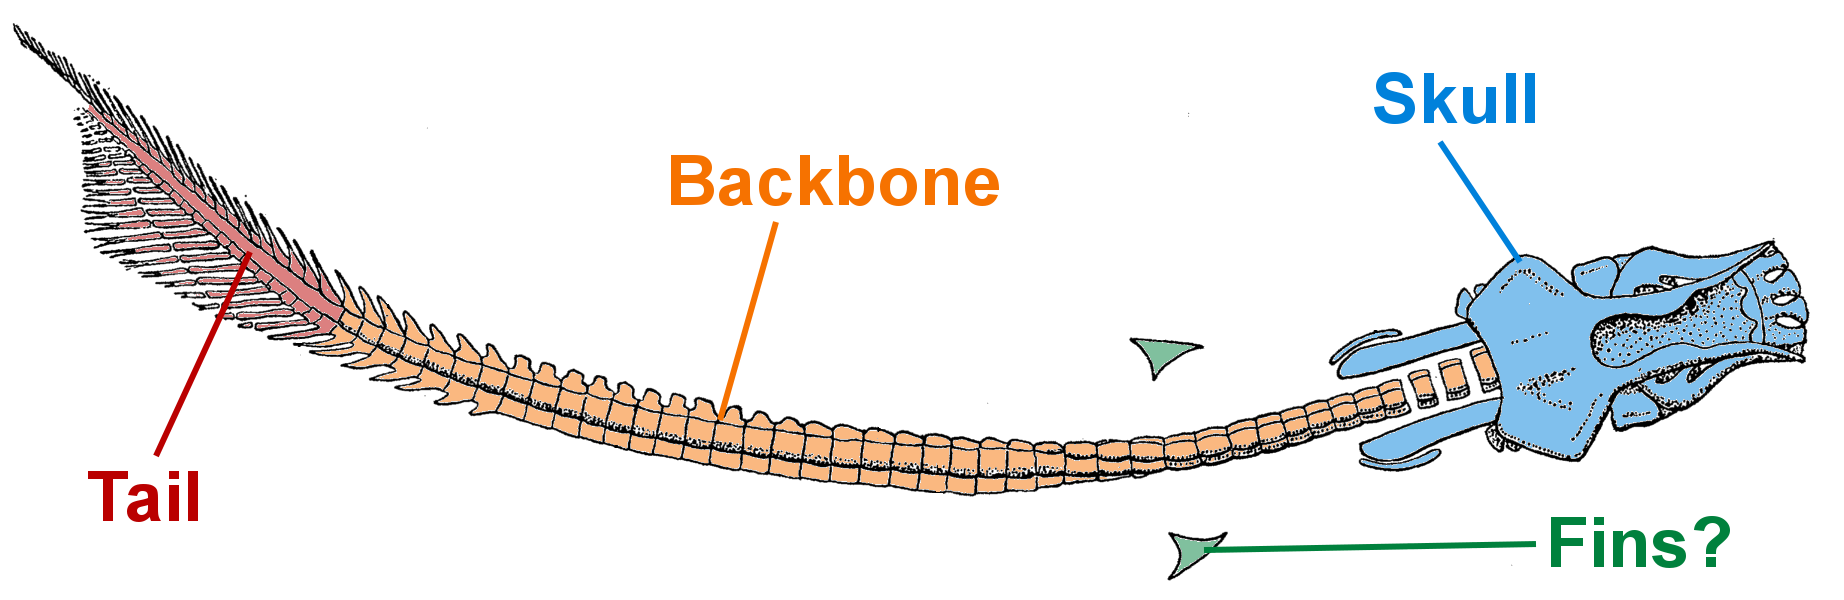
\includegraphics[scale=0.45]{Palaeospondylus}
\centering
\end{figure}

{\large\textbf{\underline{Fossil facts}}\par}

\begin{itemize}
  \item You can see very clearly in the fossil that \textit{Palaeospondylus} has a backbone.  This tells us that it is definitely a vertebrate (an animal with a backbone), like fishes and us.
  \item Part of the reason why the mystery of \textit{Palaeospondylus} has been so difficult to solve is that the bones in its head look nothing like any other Devonian fish.
\end{itemize}


\end{document}